\documentclass[conference,twocolumn,letterpaper,10pt]{ieee-sty/IEEEtran}

% Support for colors in tables
\usepackage{booktabs}
\usepackage[table]{xcolor}
% Adds support for acronyms
\usepackage[acronym]{glossaries}
% Adds support for UTF-8 text
\usepackage[utf8]{inputenc}
% Adds support for figures
\usepackage{graphicx}
% Allows to import pdf pages
\usepackage{pdfpages}
% Adds support for referencing
\usepackage{hyperref}
% Fixes references for footnotes
\usepackage[all]{hypcap}
% Allows underlined sentences to break when reaching EOL
\usepackage{soul}
% Adds support for multiple rows in a table
\usepackage{multirow}


% Generates the acronyms list
\makeglossaries

% Acronyms list
%!TEX root = ../article.tex

\newacronym{IST}{IST}{Instituto Superior T\'ecnico}
\newacronym[plural=EPEs,firstplural=Event Processing Engines (EPEs)]{EPE}{EPE}{Event Processing Engine}
\newacronym[plural=EPNs,firstplural=Event Processing Networks (EPNs)]{EPN}{EPN}{Event Processing Network}
\newacronym[plural=EPs,firstplural=Event Providers (EPs)]{EP}{EP}{Event Provider}
\newacronym[plural=EPAs,firstplural=Event Processing Agents (EPAs)]{EPA}{EPA}{Event Processing Agent}
\newacronym[plural=ECs,firstplural=Event Consumers (ECs)]{EC}{EC}{Event Consumer}
\newacronym[plural=DAGs,firstplural=Directed Acyclic Graphs (DAGs)]{DAG}{DAG}{Directed Acyclic Graph}
\newacronym{API}{API}{Application Programming Interface}
\newacronym{YAML}{YAML}{YAML Ain't Markup Language}
\newacronym{HTTP}{HTTP}{Hypertext Transfer Protocol}
\newacronym{REST}{REST}{Representational State Transfer}
\newacronym{JSON}{JSON}{JavaScript Object Notation}
\newacronym{URL}{URL}{Uniform Resource Locator}
\newacronym{IT}{IT}{Information Technology}
\newacronym{BPA}{BPA}{Business Process Automation}
\newacronym{RSS}{RSS}{Rich Site Summary}
\newacronym{SaaS}{SaaS}{Software as a Service}
\newacronym{XML}{XML}{eXtensible Markup Language}
\newacronym{DBMS}{DBMS}{Database Management Systems}
\newacronym{SOA}{SOA}{Service-oriented Architecture}
\newacronym{IFTTT}{IFTTT}{If This Then That}


% ------------------------------------------
%  ARTICLE
% ------------------------------------------

\begin{document}

% Variables file
%!TEX root = ./dissertation.tex

% Dissertation basic information
\newcommand {\Title} {Will It Blend?}
\newcommand {\StudentName} {Paulo Duarte Esperança Garcia}
\newcommand {\DegreeName} {Information Systems and Computer Engineering}
\newcommand {\MainSupervisor} {Prof. Dr. Daniel Jorge Viegas Gonçalves}
\newcommand {\SecondSupervisor} {Prof. Dra. Sandra Pereira Gama}
\newcommand {\Chairperson} {Prof. Dr. Someone}
\newcommand {\Advisor} {\MainSupervisor}
\newcommand {\CommitteeMembers} {Prof. Dr. Someone}

% Include or not include acknowledgments
\def \includeAcknowledgments{1}

% Date
\newcommand {\Month} {October}
\newcommand {\Year} {2016}

% Acknowledgments page number
\def \acknowledgmentsPage{1}

% Abstract-en page numbering
\def \abstractEnglishPage{3}

% Abstract-pt page number
\def \abstractPortuguesePage{5}

% You can define your own variables here
%\definecolor{name}{model}{color-spec}
\definecolor{red}{HTML}{FF0000}
\definecolor{green}{HTML}{00FF00}
\definecolor{blue}{HTML}{00FF00}


% Article title
\title{\Title}

% Author(s) Name
\author{\Authors}

\maketitle
\thispagestyle{plain}
\pagestyle{plain}

% Abstract
%!TEX root = ../article.tex

\begin{abstract}
  Over the last years, research has been made to ascertain if the blending
  of two or more colors can convey, in a efficient way, the information contained in two or more variables, using color blending techniques.
  Nonetheless, previous investigation has not come to an agreement. \\
  %
  With our user study, we have found that CMYK is the color model that best resembles the users’ expectations, while the orange, green and yellow color-blending results
  are the ones which generate shorter distances to between the reference colors and the ones indicated by the users. On the other hand,
  the CIE-L*C*h* Color Model is the one which is farther apart from the users’ mental model of color. We have also detected that there
  is a mild indicator that it exists a difference between the responses from Female and Male users, but only in a few color blendings.
  All the data collected was developed through a user study with 259 users, which was supported by an online user studies platform called \emph{BlendMe!}. \\
  %
  We gathered a set relevant implications of using color blending techniques, in the InfoVis field of research, besides providing a set of
  questions which remain unanswered and could turn out as an interesting source of future work, and a cleaned dataset containing the data collected
  from the user study which could be further analyzed by other researchers.
\end{abstract}


% Keywords
%!TEX root = ../article.tex

\begin{IEEEkeywords}
colors, models, spaces, blending, InfoVis, color perception, user study, calibration, scales, organization, data visualization, data processing, blending techniques, color vision deficiencies, demographic analysis
\end{IEEEkeywords}


% Sections
%!TEX root = ../dissertation.tex

% Appendix chapters entry point
% Include the chapters below

%!TEX root = ../dissertation.tex

\chapter{User Study Protocol}
\label{appendix:protocol}

\section{Motivation}
%
By conducting this first study, we intend to:
%
\begin{itemize}
  \item Conclude if there is any chance that cultural behaviours influence the user's color perception.
  \item Realize which color mixtures are more easily perceived by humans.
  \item Understand if, by using color, it is possible to clearly and easily convey information.
  This can be particularly interesting and useful when visualizing graphs or maps.
  \item Conclude if a person is capable of, not only building a mental color mixture model, but
  also deconstructing mixtures into their basic components.
\end{itemize}
%
\section{User Profiling Phase}
%
This study is anonymous and should take you up to 15 minutes. Please, answer the following answers accordingly.
%
\section{Testing Calibration Phase}
%
In this step, it's going to be presented to you a set of images. You should tune you screen definitions, in
order to answer the questions, keeping them until the end of this study. \par
%
Please, follow the steps below indicated and answer the questions.
%
\begin{enumerate}
  \item If possible, adjust your room lights for a comfortable usage of your device.
  \item Avoid reflections on your screen, by diverting the screen from direct sources of light. This step is important,
  since light reflections can affect visualization of images.
  \item To adjust the \textbf{Black Point} of your screen, define the \ul{Contrast} and \ul{Brightness} of your screen to their maximum.
  \item After Step 3, gradually reduce \textbf{Brightness} value of your screen, in order to correctly distinguish the squares of each image below [calibration squares images].
  \item If possible, define the \textbf{Color Temperature} of your screen to 6500 Kelvin Degrees.
  \item You are now ready to answer the following questions!
\end{enumerate} \par
%
\ul{NOTE:} These 6 steps are only available to the Online Users, since the Laboratory Users
do not need to perform these steps as the LCD display is already calibrated.
%
\section{Testing Color Vision Deficiences Phase}
%
This is the Color Vision Deficiencies Test. \\
%
In this step, it is going to be presented six plates with a colored pattern. Your job is to
identify the number present in each plate, typing it down in the text box below. According
to your answer, this test will inform us if you have any type of color vision deficiency which
may undermine the job of color detection. \\
%
\section{Core Test Phase}
%
Choose the Resulting color which you believe it is the result of mixing the First and Second color, by adjusting the slider below the Resulting color. \\
%
Choose two colors with which you can achieve the Resulting color, by adjusting the sliders below each color. \par
%
\ul{NOTE:} These instructions appear alternately, depending on the type of question which is shown.
%

%!TEX root = ../dissertation.tex

\chapter{Processing Data}
\label{appendix:matlab_example}
%
In this Appendix, it is available a portion of the \emph{Matlab} script which analyzed each question. Particularly, this
section analyzes the Laboratory Regular users from Question 2, which concerns the blending of Red and Blue producing Magenta. \\
%
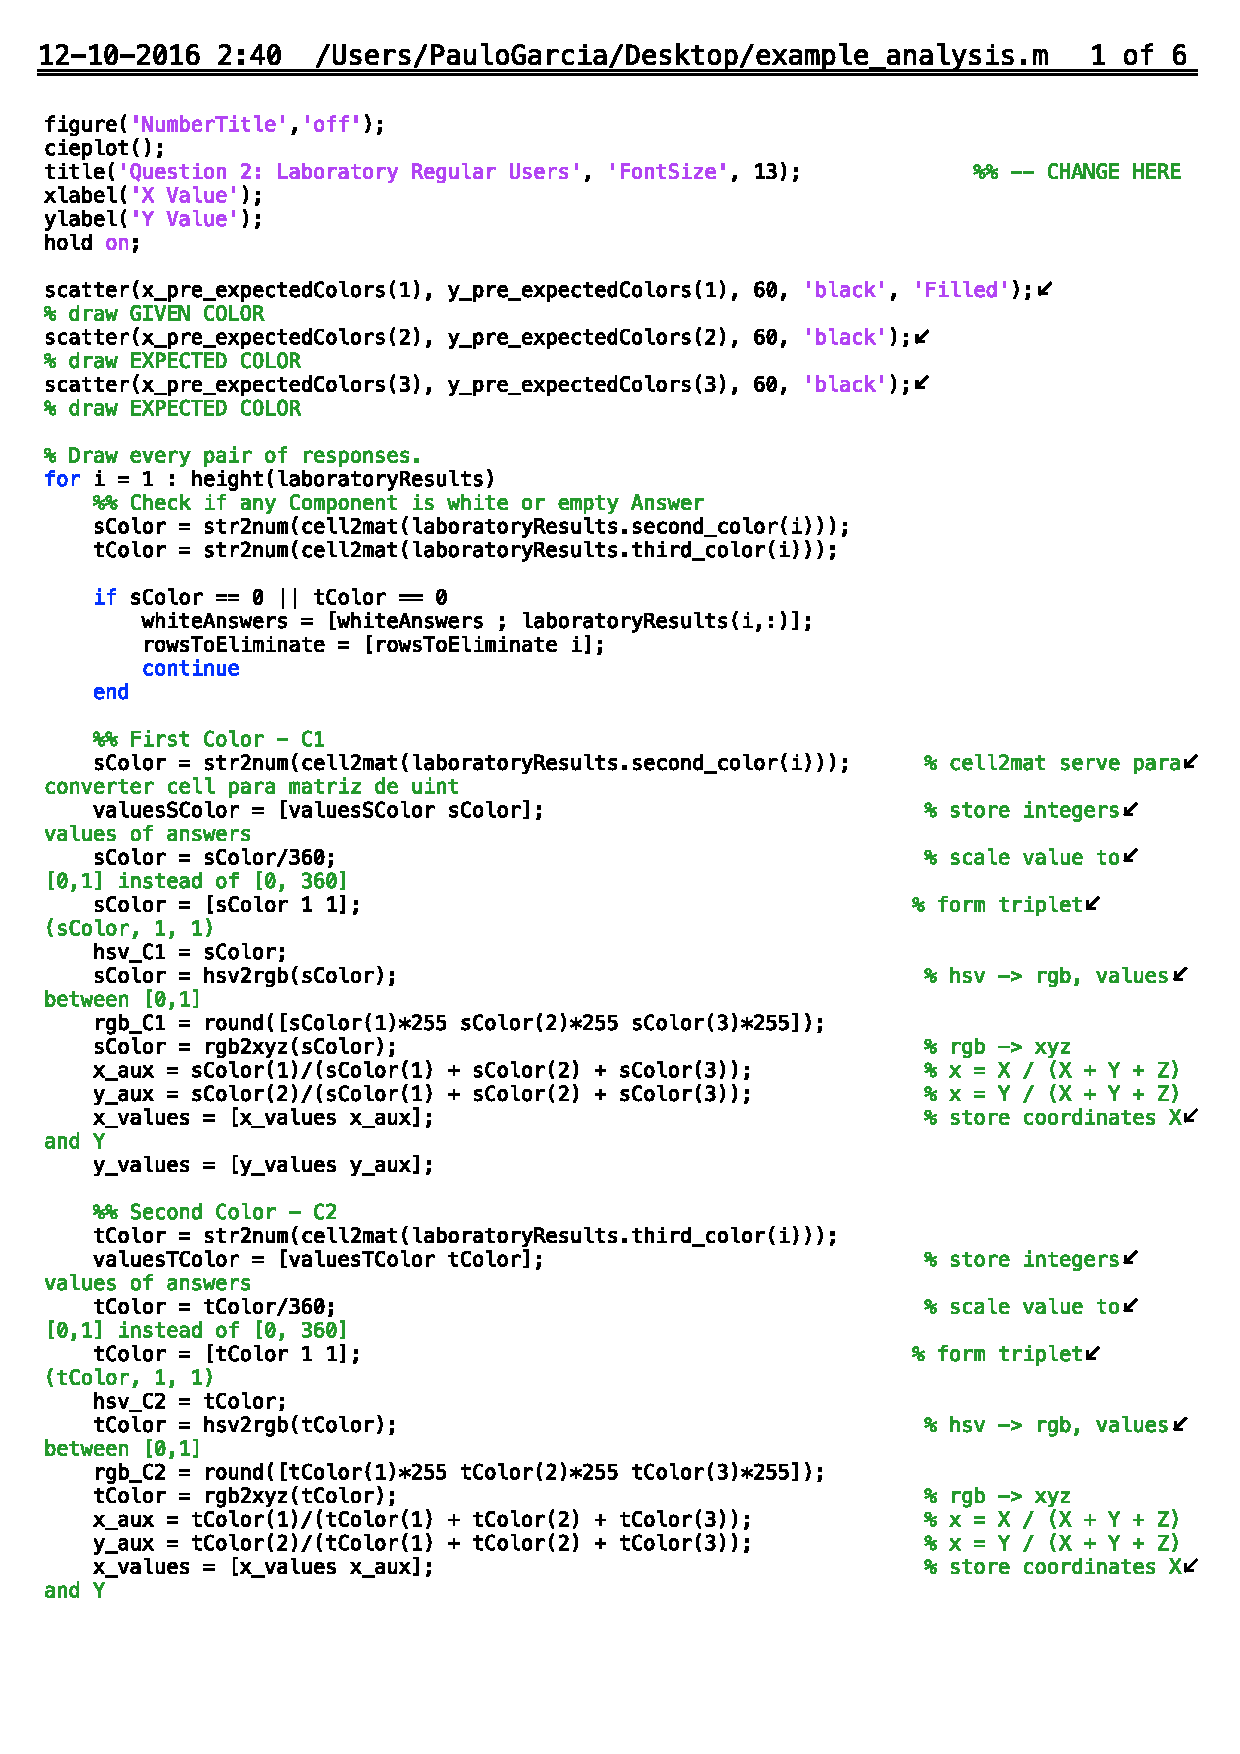
\includepdf[pages=-,pagecommand={},scale=0.88]{images/appendixes/example_analysis.pdf}

%%!TEX root = ../dissertation.tex

%%!TEX root = ../dissertation.tex

\chapter{Exercises}
\label{appendix:exercises}

Include Relevant Tables here.



% Bibliography
\bibliographystyle{IEEEtran}
% Bibliography file
\bibliography{IEEEabrv,bibliography/article}

\end{document}
